\documentclass{article}
\usepackage[utf8]{inputenc}
\usepackage[spanish,mexico]{babel}
\usepackage{listings}
\usepackage{graphicx}
\usepackage{verbatim} 
\graphicspath{ {images/} }
\usepackage{cite}

\begin{document}
	
	\begin{titlepage}
		\begin{center}
			\vspace*{1cm}
			
			\Huge
			\textbf{Segundo Parcial}
			
			\textbf{Informe de implementación}
			
			\vspace{0.5cm}
			\LARGE
			Ajuste de una imagen para visualizarla en un arreglo de LEDs con menor o mayor resolución
			
			\vspace{1.5cm}
			
			\textbf{David Correa Ochoa} 
			
			\vspace{0.8cm}
			
			\textbf{Y}
			
			\vspace{0.8cm}
			
			\textbf{Francis David Roa Bernal}
			\vfill
			
			\vspace{0.8cm}
			
			\Large
			Departamento de Ingeniería Electrónica y Telecomunicaciones\\
			Universidad de Antioquia\\
			Medellín\\
			Septiembre de 2021
			
		\end{center}
	\end{titlepage}

\tableofcontents
	\newpage
	\section{Descripción del problema}\label{intro}
	Se debe extraer la información RGB de una imagen y modificar dicha información para que por medio de varios arreglos de LEDs RGB o NeoPixel en el simulador TinkerCad se pueda visualizar la misma imagen con una menor o mayor resolución.
	
	\section{Solución implementada} \label{contenido}
	A continuación se describen las soluciones implementadas para resolver el problema descrito en la sección anterior.
	\begin{itemize}
		\item Para la reducción se implementó;
		\begin{itemize}
			\item Recorrer la fila de la imagen mientras se copia el contenido en un vector hasta que la cantidad de elementos en el vector sea adecuada, entonces se extrae un promedio de los valores contenidos en el vector, luego se guarda el promedio como un nuevo elemento en otro vector para luego borrar la información del primer vector cambiar de fila y repetir todo lo descrito hasta que se termine de recorrer la imagen.
			\item Luego de terminar de recorrer la imagen, se recorre el vector donde se guardaron los promedios y se recorre recorre de forma adecuada mientras se suman los elementos recorridos hasta alcanzar un número de elementos recorridos adecuado para calcular un promedio de los elementos recorridos y guardar el promedio como un nuevo elemento en otro vector, se repite todo lo descrito en el presente item hasta que se termine de recorrer el primer vector.
			\item El item anterior da como resultado una versión rotada en sentido anti-horario dentro del último vector, por lo que se crea un nuevo vector para guardar de forma adecuada la información del vector con la imagen rotada con el propósito de que la imagen final quede bien orientada en el nuevo vector.
		\end{itemize}
		\item Para el aumento se implementó;
		\begin{itemize}
			\item Recorrer la fila de una imagen elemento por elemento mientras se copia el contenido en un vector y se consulta la posibilidad de clonar el presente elemento, si el elemento se puede clonar entonces se vuelve a ingresar el mismo elemento en el vector la cantidad de veces que sea necesario para luego seguir con el proceso de revisión y clonado hasta llegar al último elemento de la fila para luego cambiar de fila y repetir todo lo descrito hasta terminar de recorrer la imagen.
			\item Luego de terminar de recorrer la imagen se crea un nuevo vector y se le reserva una capacidad adecuada y luego se copia en este la información contenida en el primer vector.
			\item Se recorre el nuevo vector mientras se evalúa la posibilidad de clonar una cierta cantidad de elementos que de ser posible, se copia cada elemento del grupo e insertan dentro del mismo vector a una distancia(en número de elementos) adecuada de los originales luego se repite todo lo descrito una cantidad de veces adecuada.
		\end{itemize}
	\end{itemize}
	\section{Clases implementadas} \label{Clases}
	Luego de una revisión de los ejemplos proporcionados en clase y una breve discusión se optó por utilizar las clases QImage, Adafruit\_NeoPixel y vector.
	
	\begin{itemize}
	    \item La clase QImage del entorno QT se utilizará para obtener los datos de la imagen a modificar. Se utilizaran métodos como el height(), width(), pixelcolor(), red(), blue() y green().
	    \item La clase vector del entorno QT se utilizará para guardar los datos proporcionados por QImage en vectores, generando en el algoritmo 6 vectores, 3 de uso temporal y 3 que guardaran los datos de la imagen ya modificada, estos últimos son los que se imprimirán en un archivo de texto para usarlos en Arduino.
	    \item 	La clase Adafruit\_NeoPixel del entorno Arduino se utilizará en el código de Arduino donde permitirá a través del método setPixelColor() para manipular de manera sencilla de las tiras de neopixel solo necesitando 4 datos; posición (x,y) del led y los valores de intensidad de cada RGB(rojo,verde,azul).
	    \item Se creó una clase imagen que se utiliza para guardar la información de la imagen y la dirección de la misma además de métodos que hacen uso de objetos de las clases QImage, vector y ofstream.
	    \item La clase ofstream permite, leer, escribir, crear y modificar archivos de texto.
	\end{itemize}
	
	\section{Estructura de las clases implementadas}
	Imagen: la clase imagen contiene una serie métodos que, en conjunto se encargan de;
	\begin{itemize}
	    \item obtener los datos RGB de una imagen
	    \item ajustar las dimensiones de la imagen para que se pueda mostrar en las tiras de LEDs Neo Píxel del circuito de la figura (\ref{fig:Circuito})
	    \item escribir la información de la imagen redimensionada en un archivo de texto para su posterior uso.
	\end{itemize}
	
	\section{Módulos de código}
	
\begin{lstlisting}[language=C++, label=codigo_ejemplo]

//estos son fragmentos del codigo implementado

/*
Fragmento donde se crea una instancia de la clase imagen y se pasa la
direccion de la imagen parametro a su constructor, se crea una
instancia de la clase QImage, se usa un metodo de la clase imagen que
accede a un atributo que tiene almacenado la direccion de la imagen,
se abre la imagen con un metodo de la clase QImage y se guarda en la
instancia de QImage
*/

imagen pic(a);
QImage im;
im=pic.dar_imagen();

/*
Fragmento donde se llama un metodo de una instancia de la clase imagen
para crear y/o abrir un archivo de texto
*/

pic.abrir_archivo();

/*
Fragmento donde se llama un metodo de una instancia de la clase imagen
que reduce el ancho de una imagen para un solo color varias veces para
reducir el ancho de todos los colores de la imagen, se le pasan como
parametros un char (controla la informacion de que color se va a usar) y
una instancia de la clase QImage (tiene guardada la informacion de una
imagen)
*/
pic.reduccionc(im,r);
pic.reduccionc(im,g);
pic.reduccionc(im,b);

/*
Fragmento donde se llama un metodo de una instancia de la clase imagen
que aumenta el ancho de una imagen para un solo color varias veces para
asi aumentar el ancho de todos los colores de la imagen, se le pasan
como parametros un char (controla la informacion de que color se va a
usar) y una instancia de la clase QImage (tiene guardada la informacion
de una imagen)
*/
pic.aumentoc(im,r);
pic.aumentoc(im,g);
pic.aumentoc(im,b);

/*
Fragmento donde se llama un metodo de una instancia de la clase imagen
que aumenta el largo de una imagen para un solo color varias veces para
asi aumentar el largo de todos los colores de la imagen, se le pasan
como parametros un char (controla la informacion de que color se va a
usar) y una instancia de la clase QImage (tiene guardada la informacion
de una imagen)
*/
pic.aumentof(im,r);
pic.aumentof(im,g);
pic.aumentof(im,b);

/*
Fragmento donde se llama un metodo de una instancia de la clase imagen
que reduce el largo de una imagen para un solo color varias veces para
reducir el largo de todos los colores de la imagen, se le pasan como
parametros un char (controla la informacion de que color se va a usar) y
una instancia de la clase QImage (tiene guardada la informacion de una
imagen)
*/
pic.reduccionf(im,r);
pic.reduccionf(im,g);
pic.reduccionf(im,b);

/*
Metodo que se utiliza para generar el fragmento de codigo para el proyecto de tinkercad, este es llamado al finalizar la reduccion o aumento de la imagen.Este metodo recibe un vector con uno de los colores RGB y tambien recibe un char con su respectiva letra(Rojo="r",Verde="g",Azul="b").
*/
void escribir(vector<int>,char);

Fragmento donde se llama un metodo de una instancia de la clase imagen
para crear y/o abrir un archivo de texto a partir de la clase ofstream
*/
pic.cerrar_archivo();

\end{lstlisting}

	\section{Problemas presentados durante la implementación}
	\begin{itemize}
	    \item El montaje hecho en TinkerCad al principio funcionó solo cuando se trataba de mostrar un único color
	    \item El montaje en TinkerCad funcionaba parcialmente cuando se retiraba de la configuración una parte de las tiras NeoPixel
	    \item Al aumentar la cantidad de filas de una imagen se presentaron problemas de locación de memoria cuando las imágenes presentaban cierta altura
	    \item Al reducir las filas de una imagen luego de reducir las columnas, el resultado era la imagen completa reducida pero rotada en sentido anti-horario.
	\end{itemize}

	\begin{figure}[h]
	    \centering
	    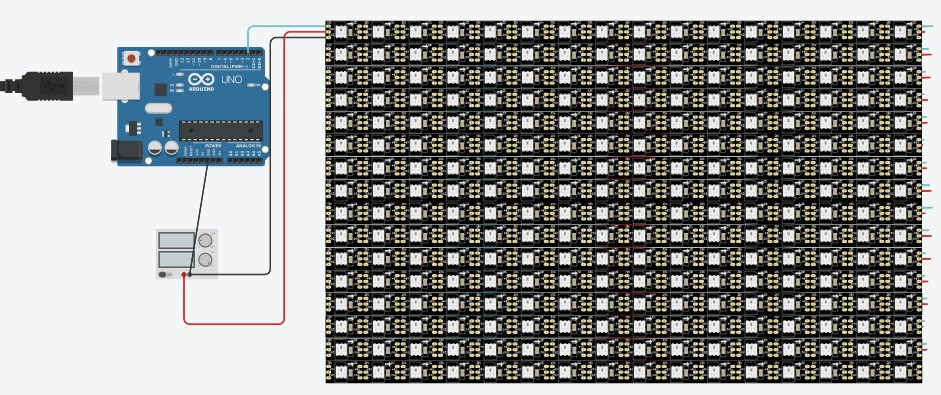
\includegraphics[width=12cm]{circuito.jpeg}
	    \caption{Montaje final del circuito}
	    \label{fig:Circuito}
	\end{figure}
\end{document}
